\section{Trigger} 
\label{sec:trigger}

Events for the signal region are collected using a set of dedicated
triggers designed to select events with large $\ptmiss$ and large $\mht$ based on
the online particle flow (PF) algorithm. In these dedicated trigger algorithms,
identified PF muons are removed from the event before the
$\ptmiss$ and the $\mht$ objects are calculated. With this definition,
the signal trigger paths can also be used to select single and double muon events for the W and Z control regions, respectively.

Electron events for the W and Z regions are selected using a single electron trigger.
To ensure the trigger efficiency also for high-$\pt$ electrons, the single electron trigger is used in combination with
a single photon trigger~\cite{CMS-EGM-TWIKI-HLT}. The same photon trigger is used to select events for the photon control region.

The full list of triggers used, along with the L1 seeds and the associated primary datasets are shown in Table~\ref{tab:triggers}.
\begin{table}[h]
    \centering
    \def\arraystretch{1.5}

    \small
    \caption{HLT paths and the associated L1 seeds used in the analysis for the 2017 and 2018 datasets. 
    The HLT paths ending in ``\_HT60'' are backup triggers introduced to mitigate noise rate problems in 2017. 
    Their inclusion is not strictly necessary for 2018, but is done for consistency.}

    \footnotesize
    \begin{tabular}{l l c c}
        \hline\hline
        Year                   & HLT path                                                  & L1 seed                         & Primary dataset               \\\hline\hline
        \multirow{5}{*}{2017}  & HLT\_PFMETNoMu120\_PFMHTNoMu120\_IDTight                  & \texttt{L1\_ETMHF70}            & MET                           \\
                               & HLT\_PFMETNoMu120\_PFMHTNoMu120\_IDTight\_PFHT60          & \texttt{L1\_ETMHF80\_HTT60er }  & MET                           \\\cline{2-4}
                               & HLT\_Ele35\_WPTight\_Gsf                                  & \texttt{L1\_SingleEG24}         & SingleElectron                \\\cline{2-4}
                               & \multirow{3}{*}{HLT\_Photon200}                           & \texttt{L1\_SingleEG30}         & \multirow{3}{*}{SinglePhoton} \\
                               &                                                           & \texttt{L1\_SingleJet170}       &                               \\
                               &                                                           & \texttt{L1\_SingleTau100er2p1}  &                               \\\hline\hline

        \multirow{11}{*}{2018} & \multirow{2}{*}{HLT\_PFMETNoMu120\_PFMHTNoMu120\_IDTight} & \texttt{L1\_ETMHF100}           & \multirow{3}{*}{MET}          \\
                               &                                                           & \texttt{L1\_ETM150}             &                               \\
                               & HLT\_PFMETNoMu120\_PFMHTNoMu120\_IDTight\_PFHT60          & \texttt{L1\_ETMHF90\_HTT60er}   &                               \\\cline{2-4}
                               & \multirow{3}{*}{HLT\_Ele32\_WPTight\_Gsf}                 & \texttt{L1\_SingleIsoEG24er2p1} & \multirow{3}{*}{EGamma}       \\
                               &                                                           & \texttt{L1\_SingleEG26er2p5}    &                               \\
                               &                                                           & \texttt{L1\_SingleEG60}         &                               \\\cline{2-4}

                               & \multirow{5}{*}{HLT\_Photon200}                           & \texttt{L1\_SingleEG34er2p5}    & \multirow{5}{*}{EGamma}       \\
                               &                                                           & \texttt{L1\_SingleJet160er2p5}  &                               \\
                               &                                                           & \texttt{L1\_SingleJet180}       &                               \\
                               &                                                           & \texttt{L1\_SingleTau120er2p1}  &                               \\
                               &                                                           & \texttt{L1\_SingleEG60}         &                               \\\hline

        \hline\hline %--------------------------------------------------------------------------------------------------------------------------      \
    \end{tabular}

    \label{tab:triggers}
\end{table}

\subsection{Efficiency measurement}
\label{sec:efficiency}

\subsubsection{$\ptmiss+\mht$ triggers}
The performance of the $\ptmiss+\mht$ triggers is measured using single muon events. The
events are selected from the SingleMuon using the \texttt{HLT\_IsoMu27} (\texttt{HLT\_IsoMu24}) 
trigger for 2017 (2018), and the offline muon is required to be well-identified and have \pt larger than 40 GeV. 
The same selection is required as for the single-muon control region used in the final fit (cf. sec. ~\ref{sec:selection_cr_1m}):

\begin{enumerate}
    \item Veto on additional leptons, photons, b jets, $\tau_{had}$ candidates.
    \item $\Delta\phi(jet,\ptvecmiss)>0.5$ for the four leading jets with $\pt>30~\GeV$.
    \item (Calo \ptmiss - PF \ptmiss) / recoil < 0.5
    \item $M_{T}(\ell,\ptmiss) < 160~\GeV$.
    \item Leading AK4 jet with $\pt>80\ GeV$, passing the tight jet ID.
    \item Subleading AK4 jet with $\pt>40\ GeV$.
    \item $\detajj > 1.0$
    \item $\dphijj < 1.5$
\end{enumerate}

To understand the dependence of the efficiencies on the jet kinematics, we measured the efficiency in three different categories:

\begin{itemize}
    \item Two central VBF jets: Leading two jets both satisfying $|\eta| \leq 2.4$
    \item Two forward VBF jets: Leading two jets both satisfying $|\eta| > 2.4$
    \item One central and one forward VBF jet: One of the leading jets is central with $|\eta| \leq 2.4$ and the other jet in the pair is forward 
    with $|\eta| > 2.4$
\end{itemize}

In these three categories, efficiencies are measured as a function of $\mjj$ and recoil, using both data and MC samples for 2017 and 2018,
seperately. Figs.~\ref{fig:eff_mjj_2017_1m}, \ref{fig:eff_mjj_2018_1m}, \ref{fig:eff_recoil_2017_1m} and \ref{fig:eff_recoil_2018_1m} show 
the results. 

Fig.~\ref{fig:eff_recoil_2017_1m} shows the efficiencies as a function of recoil in data and MC for the three categories, 
for 2017 samples, whereas Fig.~\ref{fig:eff_recoil_2018_1m} shows the efficiencies as a function of recoil in data and MC 
for the three categories, for 2018 samples. Efficiencies in double muon control region, and efficiencies in both single and double
muon regions as a function of $\mjj$ can be found in~\ref{sec:more_trigger}.

\begin{figure}[htp]
    \begin{center}
        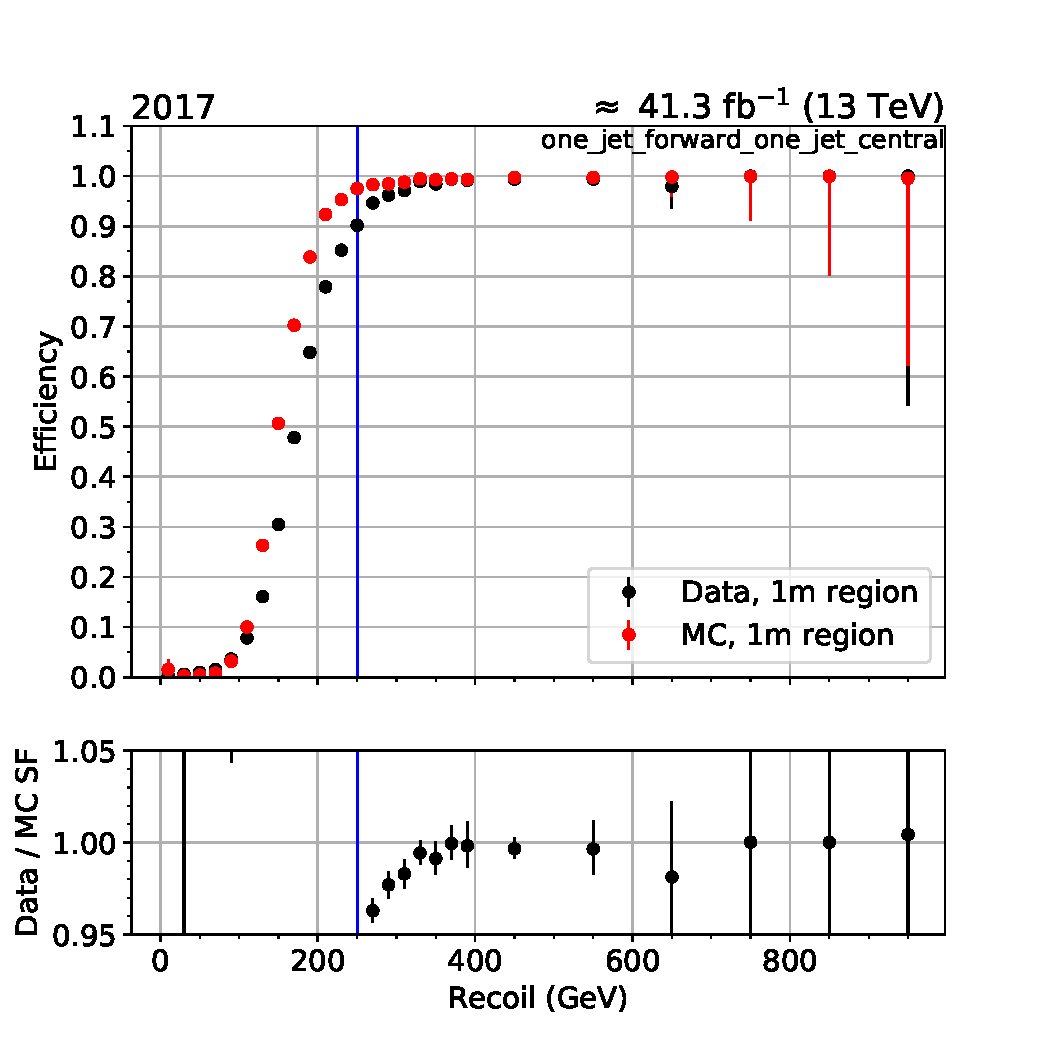
\includegraphics[width=0.49\textwidth]{fig/efficiency/trigger/met/recoil/data_mc_comparison_1m_2017_one_jet_forward_one_jet_central.pdf}
        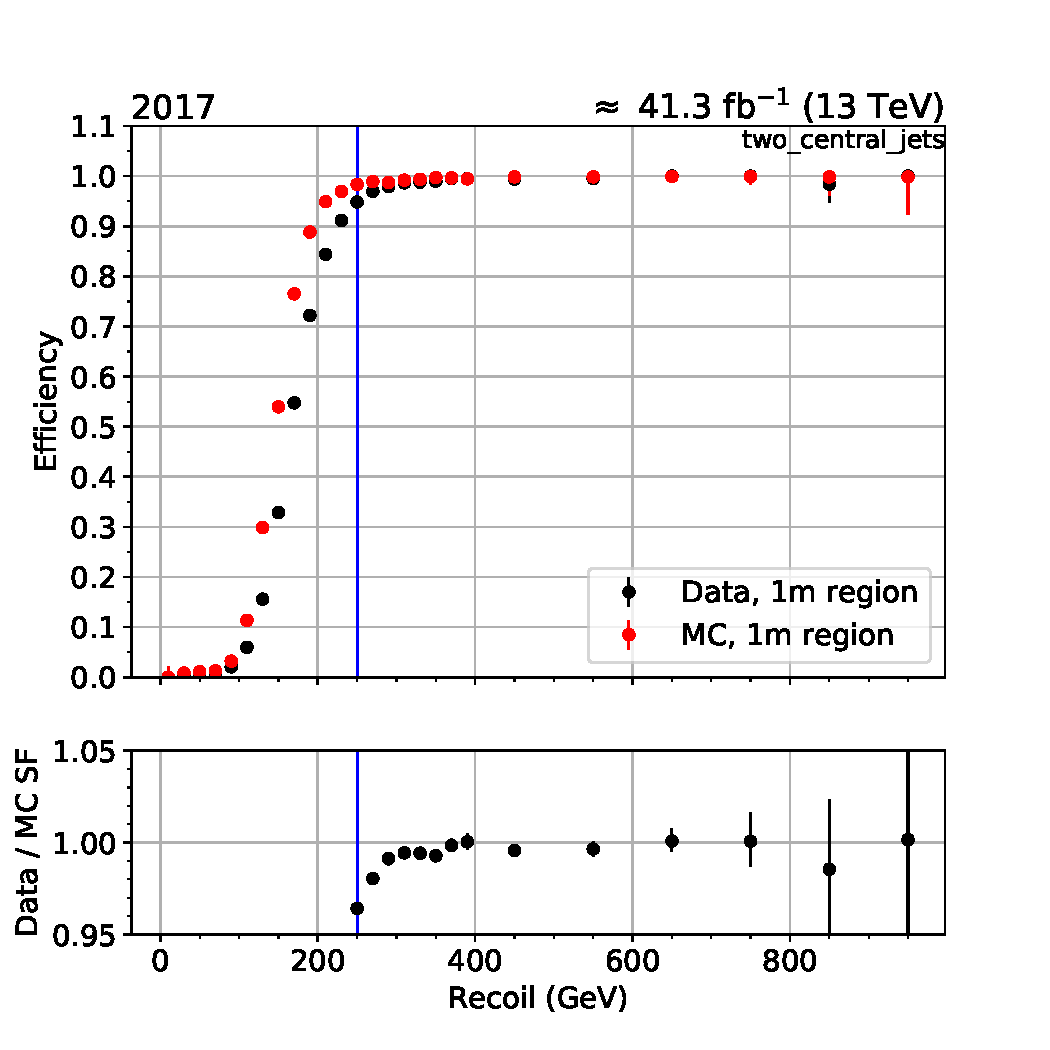
\includegraphics[width=0.49\textwidth]{fig/efficiency/trigger/met/recoil/data_mc_comparison_1m_2017_two_central_jets.pdf} \\
        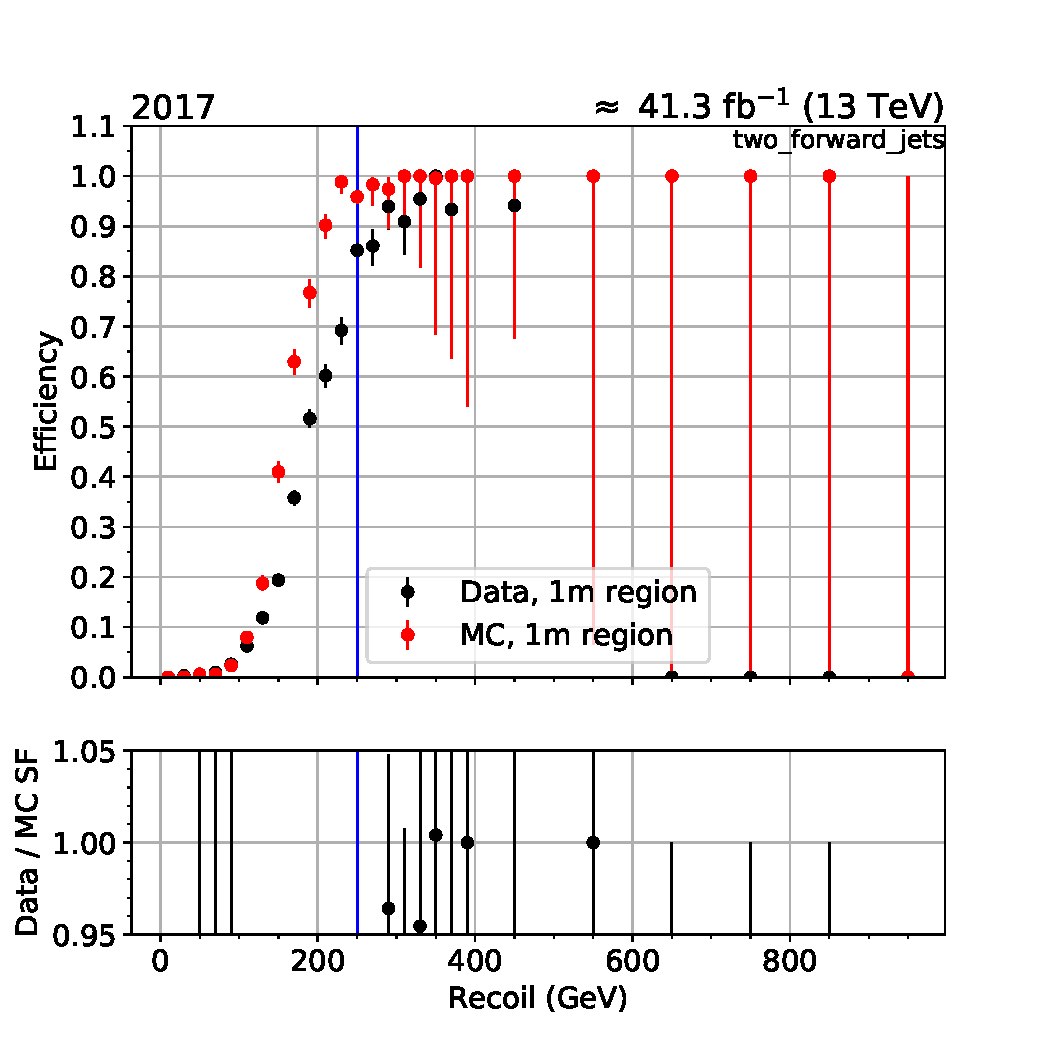
\includegraphics[width=0.49\textwidth]{fig/efficiency/trigger/met/recoil/data_mc_comparison_1m_2017_two_forward_jets.pdf}
    \end{center}
    \caption{MET trigger efficiency as a function of recoil in three categories: One forward jet and one central jet, two central jets and
            two forward jets. These results are obtained from 2017 data and MC samples with the selection of single muon events.} 
    \label{fig:eff_recoil_2017_1m}
\end{figure}

\begin{figure}[hbp]
    \begin{center}
        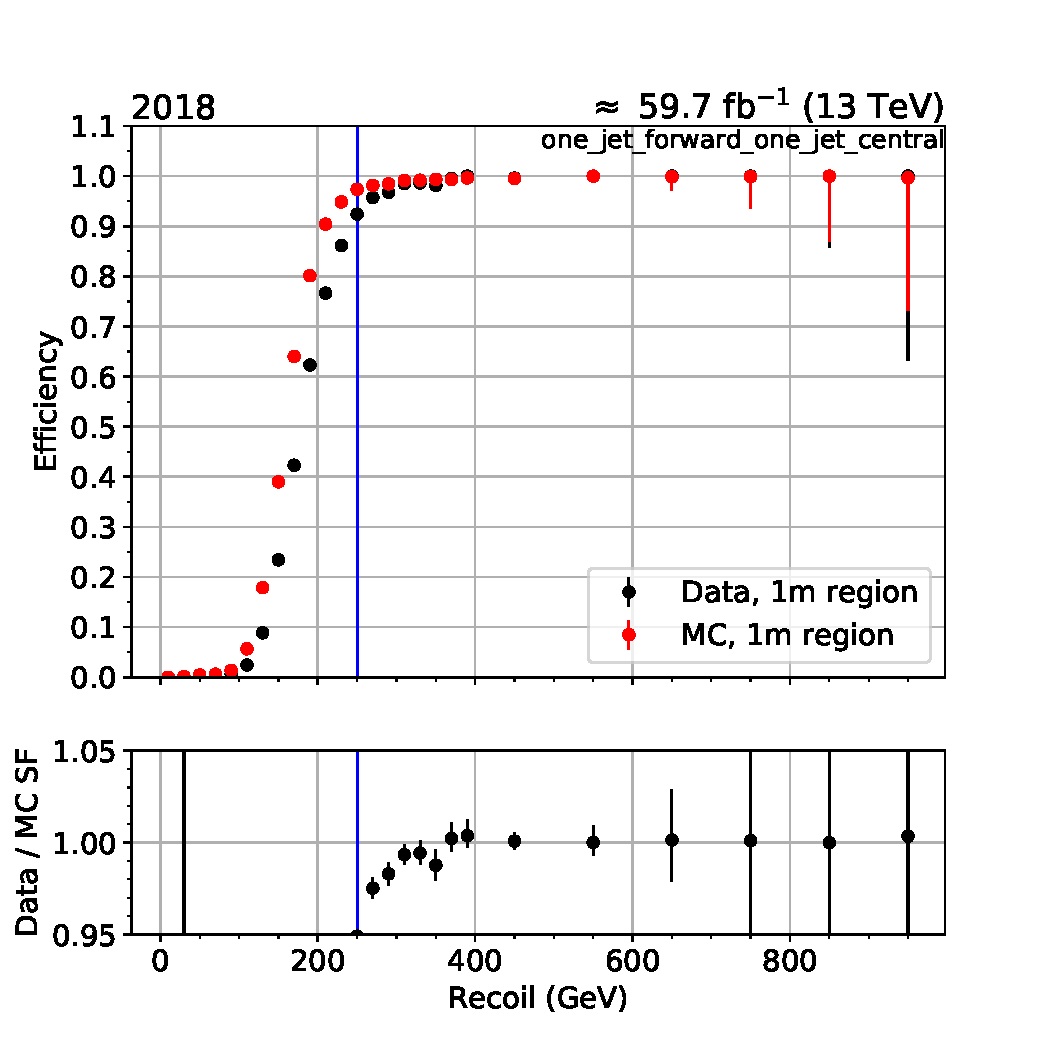
\includegraphics[width=0.49\textwidth]{fig/efficiency/trigger/met/recoil/data_mc_comparison_1m_2018_one_jet_forward_one_jet_central.pdf}
        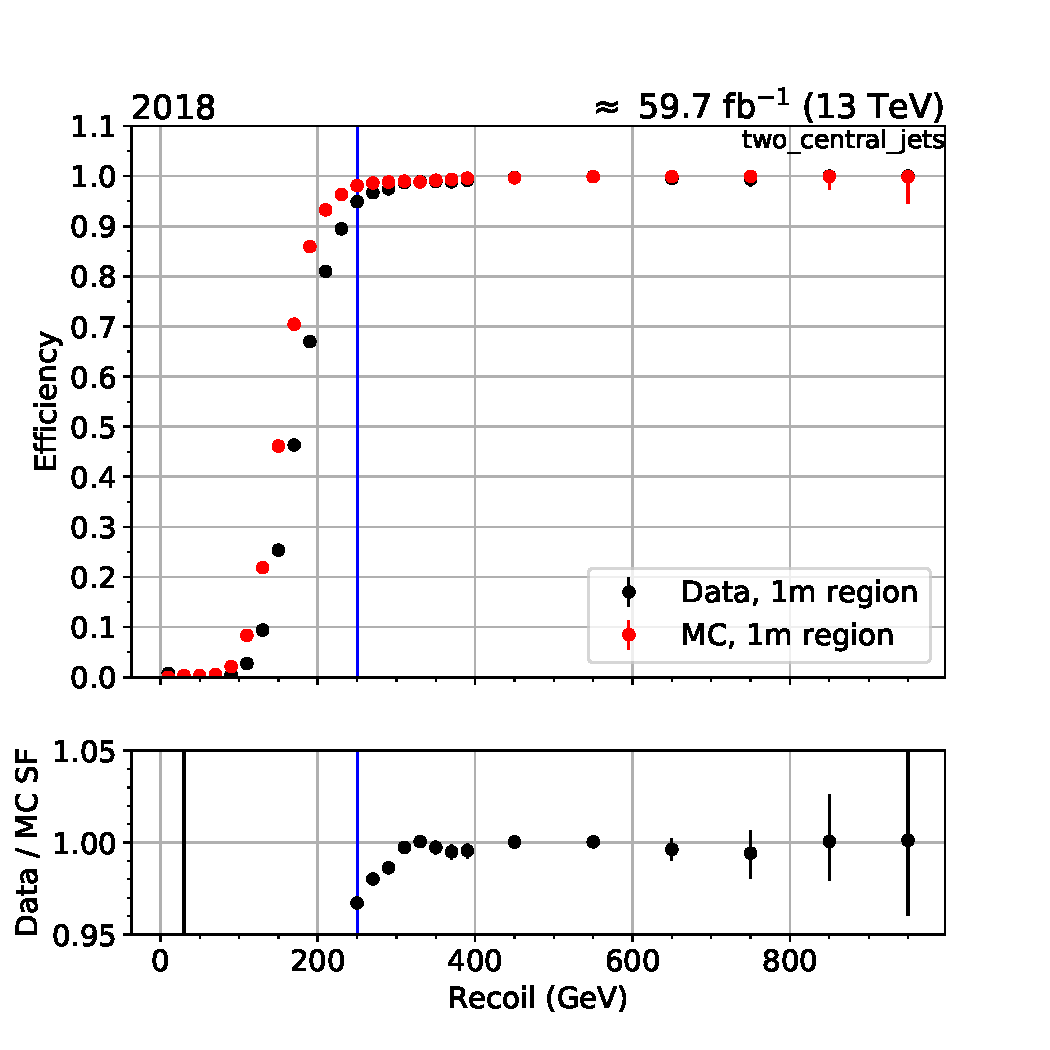
\includegraphics[width=0.49\textwidth]{fig/efficiency/trigger/met/recoil/data_mc_comparison_1m_2018_two_central_jets.pdf} \\
        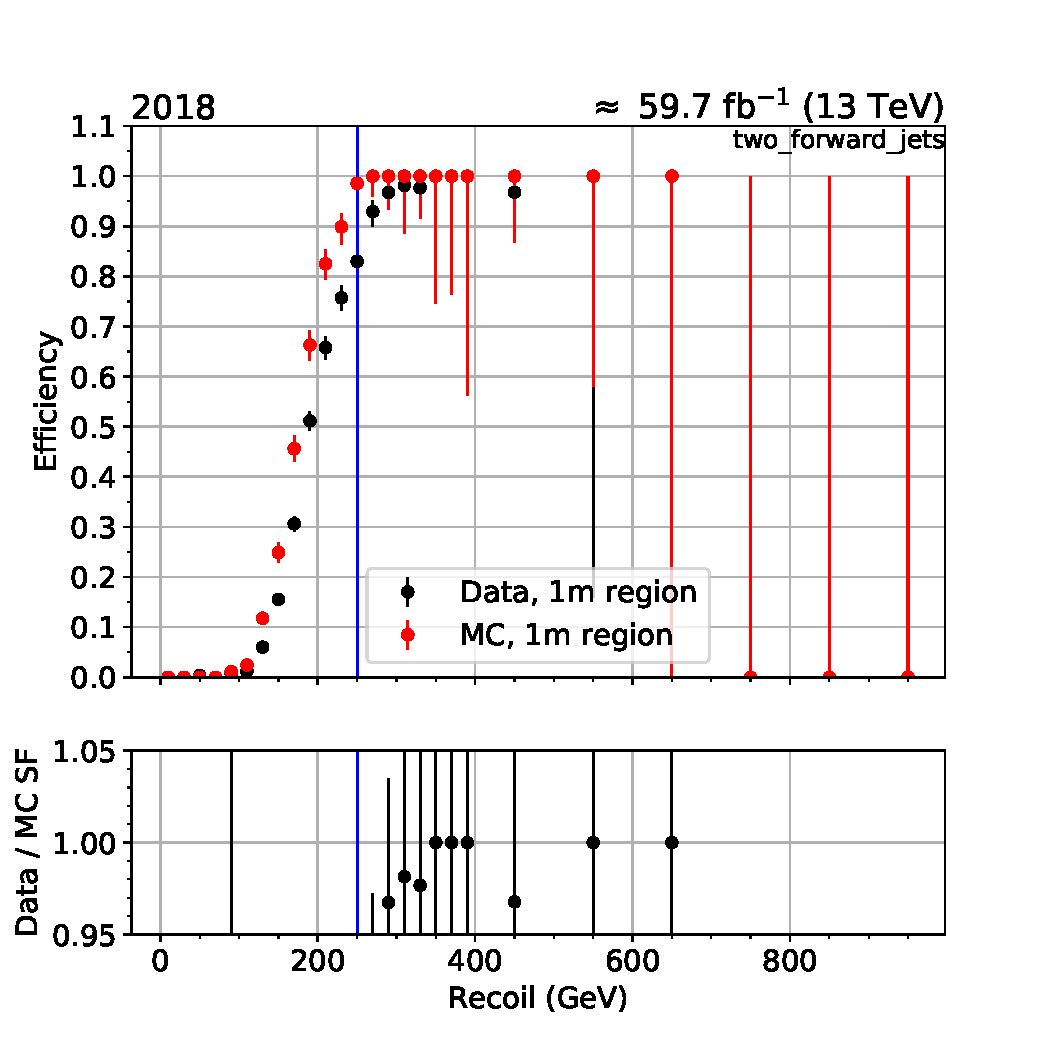
\includegraphics[width=0.49\textwidth]{fig/efficiency/trigger/met/recoil/data_mc_comparison_1m_2018_two_forward_jets.pdf}
    \end{center}
    \caption{MET trigger efficiency as a function of recoil in three categories: One forward jet and one central jet, two central jets and
            two forward jets. These results are obtained from 2018 data and MC samples with the selection of single muon events.}
    \label{fig:eff_recoil_2018_1m}
\end{figure}

Using the measured efficiencies in data and MC, data-MC scale factors are measured for the three jet kinematic cases. 
Fig.~\ref{fig:sf_recoil_1m} shows the scale factors as a function of recoil in single muon control region, using 2017 (left)
and 2018 (right) samples. We have low statistics for the two forward jets category, but overall the scale factors are close to 1.
The scale factors measured in the double muon region can be found in~\ref{sec:more_trigger}.

\begin{figure}[htbp]
    \begin{center}
        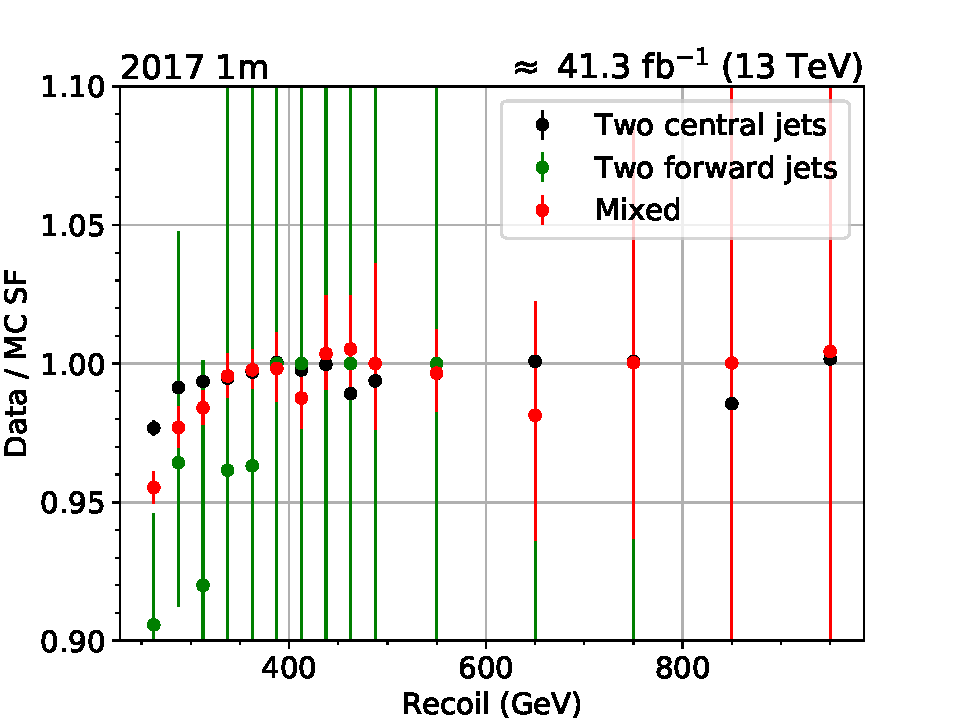
\includegraphics[width=0.49\textwidth]{fig/efficiency/trigger/met/recoil/scale_factors_1m_2017.pdf}
        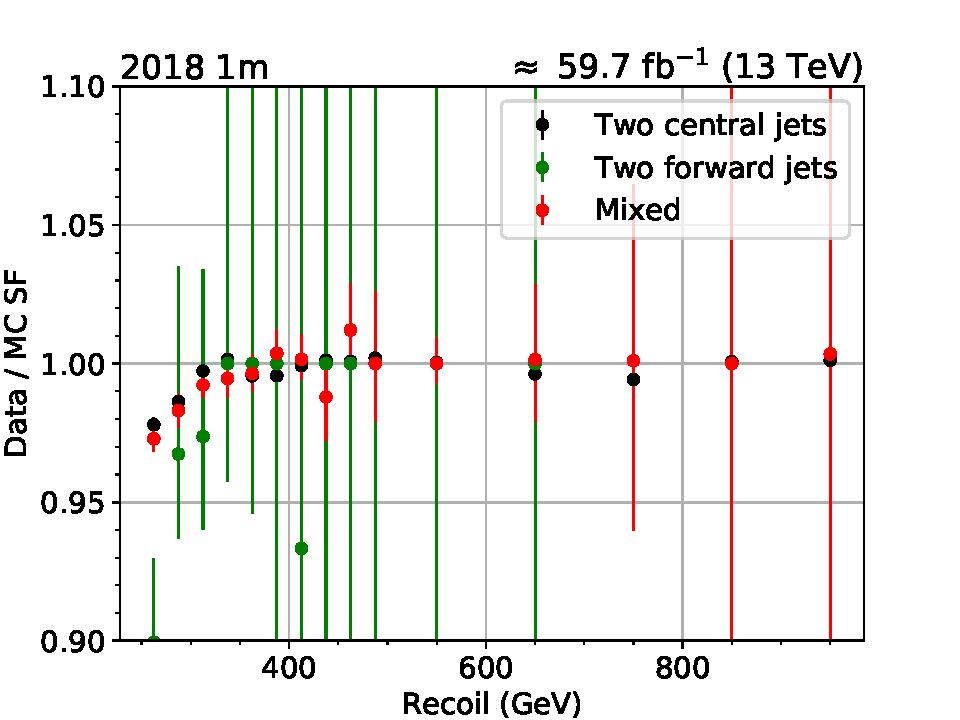
\includegraphics[width=0.49\textwidth]{fig/efficiency/trigger/met/recoil/scale_factors_1m_2018.pdf} 
    \end{center}
    \caption{Data-MC scale factors for the three jet kinematic cases in the single muon control region, using 2017 (left) and 2018 (right) samples.}
    \label{fig:sf_recoil_1m}
\end{figure}

\subsubsection{Photon trigger}
The photon trigger efficiency is measured using events from the JetHT dataset collected with the \texttt{HLT\_PFHT1050} 
trigger, which was fully unprescaled in 2017 and 2018~\footnote{The other, prescaled \texttt{HLT\_PFHTXXX} 
paths yield lower statistical precision.}. Events are selected in the same way as for the photon analysis control region 
(cf. sec.~\ref{sec:selection_cr_g}), except for the photon \pt, recoil and trigger requirements. 
The trigger efficiency $\epsilon$ is then determined as:

$$\epsilon(\texttt{HLT\_Photon200}) = \frac{\text{Offline selection \&\& \texttt{HLT\_PFHT1050} \&\& \texttt{HLT\_Photon200}}}{\text{Offline selection \&\& \texttt{HLT\_PFHT1050}}} $$

The resulting efficiency in data and \texttt{GJets} \HT-binned simulation is shown in Fig.~\ref{fig:hlteff_photon}. 
The trigger efficiency in data is larger than $95\%$ for a photon \pt of larger than $215~\GeV$, and larger than $99\%$ 
for photon \pt larger than $400~\GeV$. Between $250$ and $400~\GeV$, there is a slight inefficiency amounting to approximately 
$1\%$ at the most, with a larger amplitude in 2017 than in 2018. In both years, the turn-on behavior is almost immediate in 
simulated events, resulting in an MC-to-data scale factor almost entirely driven by the efficiency in data. 
The scale factor is within $1\%$ of unity for all bins except the lowest 2017 bin at $215\~GeV$, where is deviates 
from unity by about $4\%$.

Based on these results, the offline \pt cut for the photon in the photon control region is chosen to be $215~\GeV$.

\begin{figure*}[hbtp]\begin{center}
    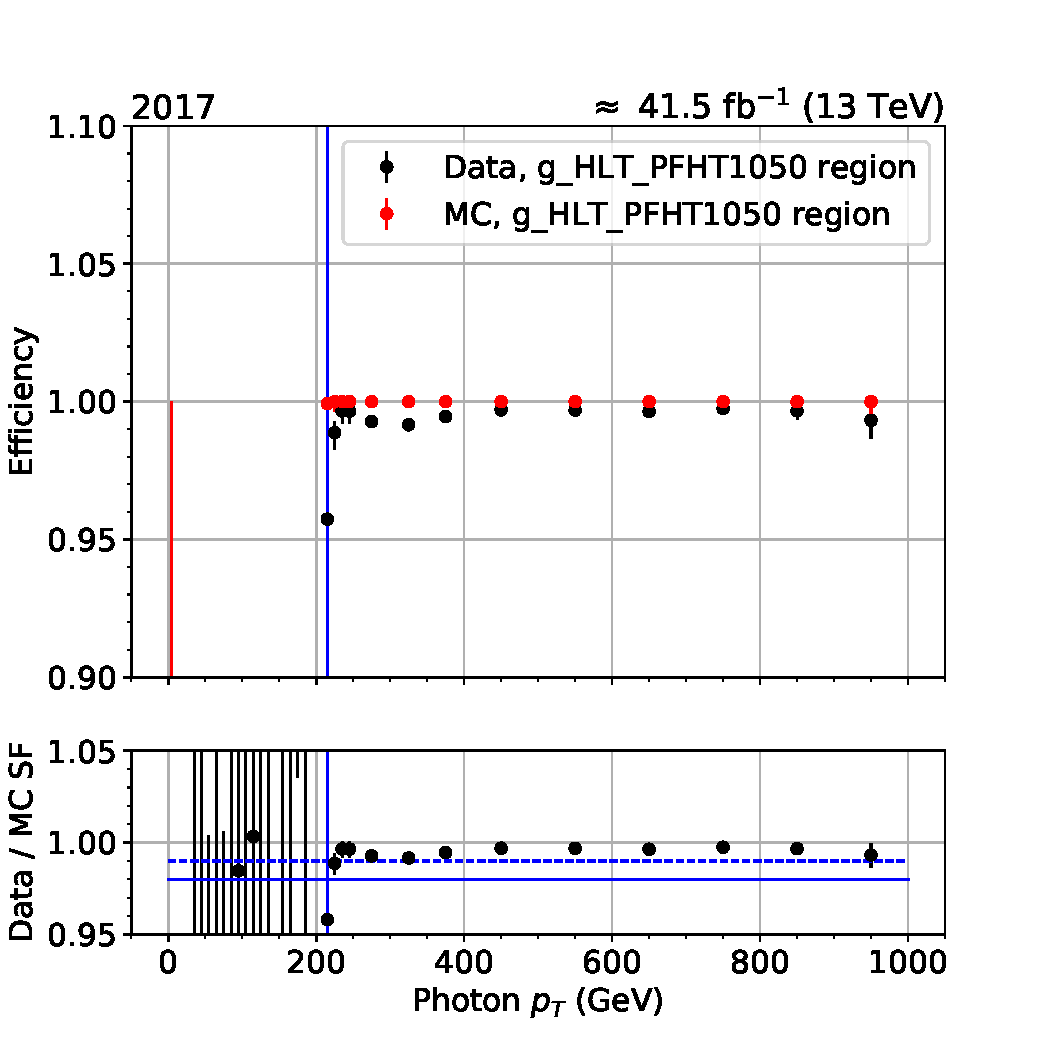
\includegraphics[width=0.49\textwidth]{fig/efficiency/trigger/photon/data_mc_comparison_g_HLT_PFHT1050_2017.pdf}
    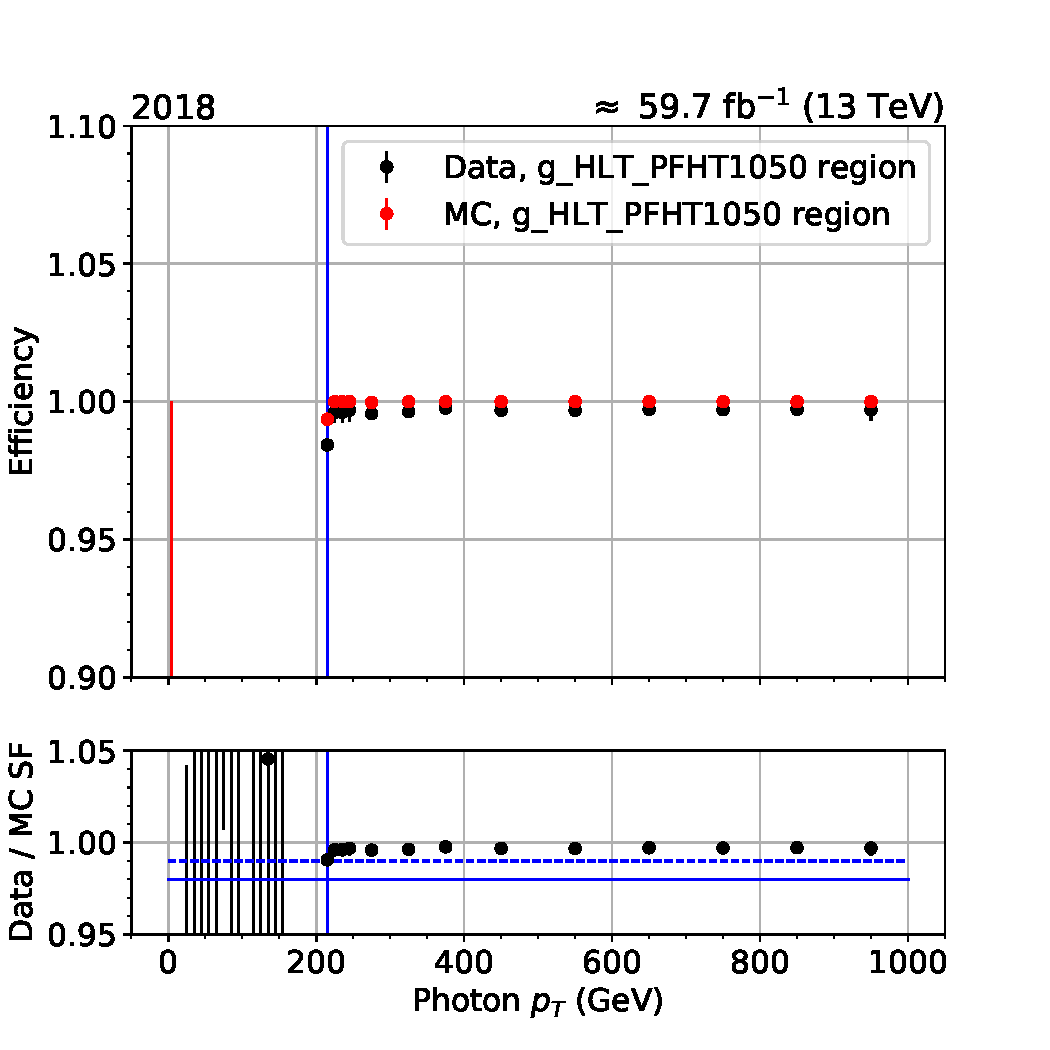
\includegraphics[width=0.49\textwidth]{fig/efficiency/trigger/photon/data_mc_comparison_g_HLT_PFHT1050_2018.pdf}
    \caption{Efficiency of the \texttt{HLT\_Photon200} trigger in data (black) and \HT-binned \texttt{GJets} simulation (red) for 2017 (left) and 2018 (right) as a function of photon \pt. The bottom panel shows the MC-to-data efficiency scale factor. The blue vertical line indicates a photon \pt of $215~\GeV$, which is the requirement used in the analysis selection.}
    \label{fig:hlteff_photon}
 \end{center}\end{figure*}

 \subsubsection{Electron trigger}
{\color{red} We also need to add information about the single electron trigger efficiencies}
